\newpage
\restoregeometry
\section{Grundlagen}
\subsection{Radarfernerkundung}
Bei der Radarfernerkundung werden vom Radarsystem elektromagnetische Impulse ausgesandt und deren Reflektionen, auch Backscatter genannt, empfangen und 
verarbeitet. Daher gehört die Radarfernerkundung zu den aktiven Fernerkundungsmethoden da hier im Gegensatz zur optischen Fernerkundung nicht nur 
von Oberflächen reflektierte Strahlung von anderen Strahlungsquellen wie der Sonne aufgenommen wird, sondern das Fernerkundungssystem 
selbst als Strahlungsquelle dient. Messungen können daher tageszeitunabhängig erfolgen. Dabei können die sendenden und erfangenden Komponenten unterschiedlich (bi- oder multistatisches Radar) oder 
identisch sein (monostatitsches Radar). Trifft der ausgesandte Impuls auf eine Oberfläche, zum Beispiel die Erdoberfläche, wird nur ein Teil des Signals 
reflektiert und vom Fernerkundungssystem empfangen \cite{tutorial_on_sar}. 

Die Eigenschaften dieses empfangenen Signal hängen sowohl von Parametern des Aufnahmesystems als von Parametern der reflektierenden Oberfläche ab.
So werden in der Radarfernerkundung verschiedenen Frequenzbänder verwendet, welche sich in Frequenz und Wellenlänge unterscheiden. 
Mit einer größeren Wellenlänge kann ein Medium tiefer durchdrungen werden. Außerdem werden Wolken, Dunst und Rauch durchdrungen was den zusätzlich Vorteil bietet
wetterunabhängig Messungen durchführen zu können \cite{einfuehrung_in_fernerkundung}. Gängige in der Radarfernerkundung verwendete Frequenzbänder können Tabelle x entnommen werden. 

\begin{table}[htb]
    \caption{Gängige Frequenz-Bänder in der Radarfernerkundung}
\begin{center}
    \begin{tabular}{|c|c|c|c|c|c|c|c|} 
        Frequenzband & Ka & Ku & X & C & S & L & P\\ 
        \hline
        Frequenz (GHz) & 40-25 & 17.6-12 & 12-7.5 & 7.5-3.75 & 3.75-2 & 2-1 & 0.5-0.25\\ 
        Wellenlänge (cm) & 0.75–1.2 & 1.7–2.5 & 2.5–4 & 4–8 & 8–15 & 15–30 & 60–120\\ 
    \end{tabular}
    \label{table:1}
\end{center}
\end{table}

Die Durchdringung hängt auch von der Dielektrizitätskonstante der reflektierenden Materialen ab. Ist diese groß, reflektiert die Oberfläche stark und die Durchdringung ist gering.
Zusätzlich ist die Polarisation der ausgesandten und empfangenen Signale bei der Messung ausschalgebend. Sie können horizontal oder vertikal polarisiert sein. Dies führt zu vier möglichen 
Polarisationsmodi für das Senden (transcieve) und das Empfangen (receive) nämlich HH, VV, HV und VH.
Der Depressionswinkel der Antenne nimmt direkten Einfluss auf die geometrische Auflösung quer zur Flurrichtung (Range Resolution) da dadurch die Dauer eines ausgestrahlten Signals
beeinflusst wird. Die geometrische Auflösung in Flugrichtung (Azimut Resolution) wiederum wird von der Länge der Sendeantenne und ihrem Abstrahlwinkel beeinflusst. Die Antennenlänge kann Bauartbedingt 
nicht beliebig gesteigert werden \cite{einfuehrung_in_fernerkundung}. So aufgenommene Daten haben also keine Quadratische Auflösung. Die tatsächliche Ausdehnung der Objekte quer zu Flugrichtung (Ground-Range) 
wird verzerrt wiedergegeben (Slant-Range). Die breite des Aufnahmegebietes (swath width) ist gleich der Ausdehnung der Ground-Range. Die Länge ergibt sich aus dem Zeitraum, indem das Radar eingeschaltet ist \cite{tutorial_on_sar}.

Plattformen, welche mit Radarsystemen mit synthetischer Apertur ausgerüstet sind, werden seit den 1980er Jahren als 
Mittel der Fernerkundung eingesetzt. Diese Systeme mit verhältnismäßig kurzen Antennen mit breitem Abstrahlwinkel ausgestattet. Durch die Bewegung der Plattform entlang 
des Azimuts kann die wirksame Antennenlänge (synthetisch) vergrößert und die empfangenen Signale miteinander korreliert werden um so eine hohe geometrische Auflösung zu erzielen \cite{tutorial_on_sar}\cite{einfuehrung_in_fernerkundung}.

\begin{figure}[h]
    \centering
    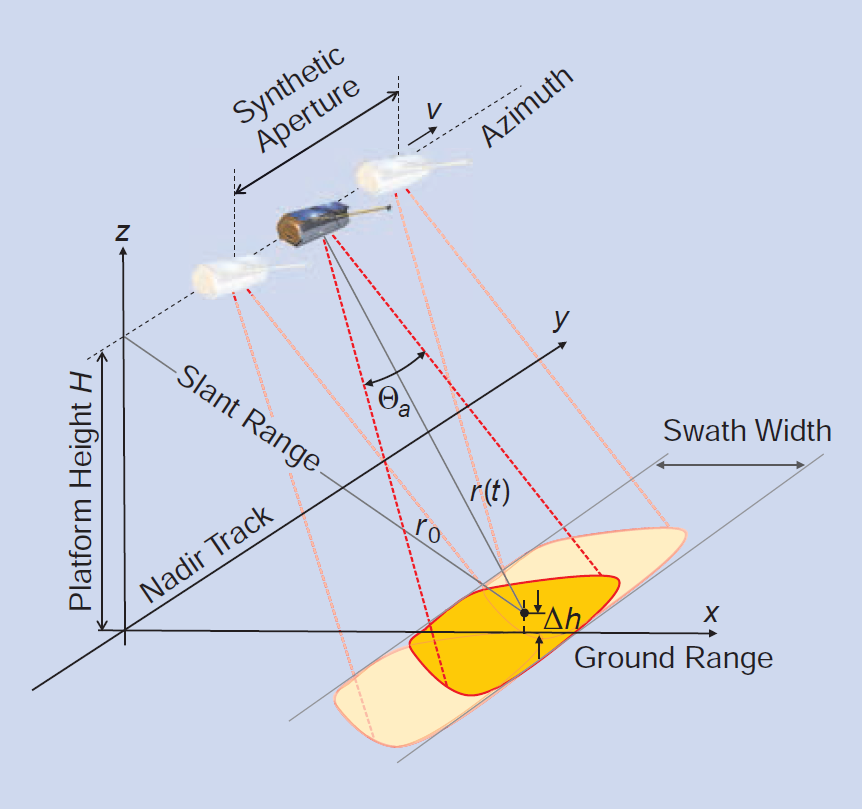
\includegraphics[width=12cm]{Bilder/SAR_Prinzip.png}
    \caption{Prinzip des Synthetic Aperture Radar - Quelle: \cite{tutorial_on_sar}}
    \label{fig:sar_prinzip}
\end{figure}

Die Rauigkeit ist eine Eigenschaft der reflektierenden Oberfläche und hat großen Einfluss auf das reflektierte Signal. Ist diese im Verhältnis zu verwandten
Wellenlänge gering so kommt es zur Spiegelung und nur ein geringer bis kein Anteil des kehrt zum Empfänger zurück. Doch auch die Form und Exposition der Oberfläche nimmt 
Einfluss auf das reflektierte Signal. So werden Flächen unterschiedlich stark bestrahlt. Ist eine dem System abgewandte Fläche steiler geneigt als der Depressionswinkel liegen Sie
sogar im Radarschatten und werden gar nicht bestrahlt \cite{einfuehrung_in_fernerkundung}. 
Im Gegensatz zu optischen Aufnahmeverfahren liefern die Rohdaten einer Befliegung mit Radarsensoren noch keine Bilddaten. Um Bilder zu erzeugen, bedarf es zunächst einer komplexen
Verarbeitung. Dabei werden die Daten entlang der Range- und Azimut-Dimension gefiltert. In der Regel repräsentieren die Pixelwerte eines aus Radardaten abgeleiteten Bildes der 
Reflektivität der korrespondierenden Fläche. Mittels Geocodierung kann das so entstandene Bild verortet werden.
Zusätzlich können diverse Kalibrierungen vorgenommen werden. Dazu gehören Verfahren welche Rauscheffekte minimieren, die geometrischen Eigenschaften verbessern oder die Interpretation
der Bilder erleichtern \cite{tutorial_on_sar}. 

\subsection{Copernicus Programm}
\subsubsection{Ziele}
\subsubsection{Sentinel 1}
\subsubsection{Datenzugang}
\subsection{Überschwemmungsmonitoring}
\subsection{Schnittstellen}
\subsection{OGC und OGC Standards}
\subsection{OGC API - Processes - Part 1: Core}
\subsubsection{Ziele}
\subsubsection{Aufbau}
\subsection{Evaluationskriterien}